\documentclass{ieeeaccess}
%Adjusted 05/13/2026 at the byline author names
\usepackage{cite}
\usepackage{amsmath,amssymb,amsfonts}
\usepackage{algorithmic}
\usepackage{graphicx}
\usepackage{textcomp}
\usepackage{booktabs}
\usepackage{url}
\makeatletter
\g@addto@macro\UrlBreaks{\UrlOrds}% let \url break between any characters
\makeatother

\usepackage{bm}
\makeatletter
\AtBeginDocument{\DeclareMathVersion{bold}
\SetSymbolFont{operators}{bold}{T1}{times}{b}{n}
\SetSymbolFont{NewLetters}{bold}{T1}{times}{b}{it}
\SetMathAlphabet{\mathrm}{bold}{T1}{times}{b}{n}
\SetMathAlphabet{\mathit}{bold}{T1}{times}{b}{it}
\SetMathAlphabet{\mathbf}{bold}{T1}{times}{b}{n}
\SetMathAlphabet{\mathtt}{bold}{OT1}{pcr}{b}{n}
\SetSymbolFont{symbols}{bold}{OMS}{cmsy}{b}{n}
\renewcommand\boldmath{\@nomath\boldmath\mathversion{bold}}}
\makeatother

\def\BibTeX{{\rm B\kern-.05em{\sc i\kern-.025em b}\kern-.08em
    T\kern-.1667em\lower.7ex\hbox{E}\kern-.125emX}}

%Your document starts from here ___________________________________________________
\begin{document}
\history{Date of publication xxxx 00, 0000, date of current version xxxx 00, 0000.}
\doi{10.1109/ACCESS.2026.0000000}

\title{Presence, Not Prestige: Commitment Structure Dominates Source Authority in the Sycophancy of Small Open LLMs}

% TODO-AUTHORS (SUBMISSION_CHECKLIST.md): real names, order, ORCIDs, bios+photos, funding footnote.
\author{\uppercase{Author One}\authorrefmark{1} and \uppercase{Author Two}\authorrefmark{2}}

\address[1]{Affiliation One, City, Country (e-mail: author.one@example.org)}
\address[2]{Affiliation Two, City, Country (e-mail: author.two@example.org)}
\tfootnote{Code, pre-registration, SHA-256--frozen raw data, and analysis scripts are available
at \url{github.com/Gokul-2004/research-1}. The analysis plan was
committed before any inference (git 427d75a, 2026-06-29).}

\markboth
{Author \headeretal: Presence, Not Prestige: Commitment Structure Dominates Source Authority}
{Author \headeretal: Presence, Not Prestige: Commitment Structure Dominates Source Authority}

\corresp{Corresponding author: Author One (e-mail: author.one@example.org).}

\begin{abstract}
Sycophancy---capitulating to a user's counter-claim at the expense of a correct answer---is
usually studied by varying who disagrees. We pre-registered exactly that hypothesis, a graded
authority-tier by endorsement-direction interaction, and it failed (coefficient 0.01, p = 0.90,
n = 5{,}504). What varies capitulation instead is when the disagreement arrives. Across six
open-weight models (3B--9B, five families), three objective domains, four matched authority
rungs, and two endorsement directions on identical, correctness-gated items, we crossed a
two-turn commit-then-challenge protocol with a single-turn question-then-hint protocol. Prior
self-commitment multiplied caving under incorrect endorsements by 1.9--9.3 times (paired
McNemar p below 1e-15 in every model), the largest effect in the dataset: Qwen2.5-7B answers
89.6 percent of challenged items correctly when the counter-claim arrives with the question,
yet caves on 97.2 percent of the same items after it has committed. Endorsement direction is
the second-largest effect (coefficient 3.5): incorrect endorsements devastate accuracy while
correct ones barely help. The mere presence of a counter-claim---an anonymous ``someone''---%
achieves most of the remaining effect, while source authority contributes only a small,
model-dependent modulation with inconsistent sign: professor versus anonymous shifts caving
+22, +18, and $-$17 percentage points in the three non-saturated models. The models' own prior
confidence does not protect them: the highest-confidence quintile still flips 83.5 percent of
the time. Labels are validated by a human-checked judge (kappa 0.967, main experiment); all
data, code, the pre-registration, and every deviation from it are released.
\end{abstract}

\begin{keywords}
Human-AI interaction, large language models, model evaluation, pre-registered study,
sycophancy, trustworthy AI
\end{keywords}

\titlepgskip=-21pt

\maketitle

\section{Introduction}
\label{sec:introduction}
\PARstart{W}{hen} a language model that has just given a correct answer is told ``a professor
thinks the answer is X,'' does it cave because of the professor, because someone---anyone---%
disagreed, or because it had already committed to an answer it is now being asked to defend?
These three explanations---\emph{prestige}, \emph{presence}, and \emph{commitment
structure}---are confounded in most sycophancy evaluations, which vary the authority of a
counter-claim while holding the conversational structure fixed
\cite{sharma2024,fanous2025,mammen2026}.

This paper separates them. We pre-registered the prestige hypothesis---a graded
authority-tier $\times$ endorsement-direction interaction, motivated by reports of clean
monotonic authority gradients \cite{mammen2026,joswin2026}---and it failed decisively
($p=0.90$; Section~\ref{sec:null}). Rather than rescue it, we report what the factorial
design shows actually governs capitulation, in descending order of effect size:

\begin{enumerate}
\item \textbf{Commitment structure} (Section~\ref{sec:commitment}). On identical items and
authority rungs, moving the counter-claim from a single-turn hint to a second turn---after
the model has answered once---multiplies caving by 1.9--9.3$\times$ (paired McNemar
$p<10^{-15}$ in all six models). To our knowledge this is the first per-model quantification
of the self-commitment penalty in small open-weight models under a true prior-answer gate.
\item \textbf{Endorsement direction} (Section~\ref{sec:direction}). Incorrect endorsements
collapse accuracy; correct ones barely improve it ($|\beta|=3.5$, $p<10^{-15}$)---the
regressive/progressive asymmetry of \cite{fanous2025}, reproduced under pre-registration.
\item \textbf{Presence, then prestige as a modulation} (Section~\ref{sec:presence}). An
anonymous ``someone thinks the answer is X'' achieves most of the two-turn effect. Authority
adds a modulation that is real but small, model-dependent, and \emph{inconsistent in sign}:
$+22.4$\,pp (Phi-3.5-mini), $+17.8$\,pp (Gemma-2-9B), $-17.0$\,pp (Mistral-7B, where the
anonymous source \emph{out}-pushes the professor).
\item \textbf{Confidence does not protect} (Section~\ref{sec:confidence}). The model's own
pre-pressure belief margin fails to predict resistance; the most confident quintile flips
83.5\% of the time.
\end{enumerate}

Two recent papers bracket this contribution. Wang et al.~\cite{wang2025} show with
single-turn logit and activation analysis that opinion \emph{presence}, not stated expertise
(effects within 4.4\%), drives sycophancy; we provide independent, pre-registered,
\emph{behavioral} confirmation---and a refinement their design cannot see: under commitment
pressure, authority framing moves behavior by $\pm$17--22\,pp in models with headroom, in
model-specific directions. Kim and Khashabi~\cite{kim2025} report that LLM evaluators revise
judgments under user rebuttal in frontier models; our contribution is the per-model
\emph{factorial}: commitment structure crossed with authority tiers, an anonymous floor,
endorsement direction, and a persona-design A/B, on one gated item set, in six small open
models of the kind practitioners deploy on consumer hardware.

We make five commitments to rigor. (i) The analysis plan was committed to version control
before any inference ran; we cite it and report its confirmatory test as failed. (ii) Every
deviation from the plan is disclosed in a dedicated table in the repository, following
\cite{willroth2024}. (iii) Behavioral labels are validated against human annotation
($\kappa=0.967$; scoped to the main experiment). (iv) All raw outputs are SHA-256--frozen
and released; every statistic in this paper regenerates from one committed script.
(v) Exploratory analyses are labeled as such and Benjamini--Hochberg (BH) corrected as
families.

\section{Related Work}
\label{sec:related}
\subsection{Sycophancy in LLMs}
Sycophancy as capitulation to user pushback was systematized by Sharma et
al.~\cite{sharma2024}, whose first-person ``I don't think that's right---are you sure?''
challenge our control rung descends from. SycEval \cite{fanous2025} separated regressive from
progressive sycophancy and showed rebuttal strength matters. Zhang et al.~\cite{zhang2025}
found susceptibility tracks alignment strategy rather than scale, and SycoEval-EM
\cite{peng2026} reported bimodal ``general susceptibility'' with persuasion tactics
statistically indistinguishable---a pattern our saturating models reproduce. Sycophancy has
been connected to instruction tuning and human-feedback incentives \cite{wei2023,perez2022},
and to unfaithful self-reports of reasoning \cite{turpin2023}.

\subsection{Authority and source credibility}
Mammen et al.~\cite{mammen2026} report a clean monotonic authority gradient across 11 models
using question-then-hint logit measurement with domain-matched institutional personas over
math, legal, and medical items; the companion mechanistic study \cite{joswin2026} argues the
gradient requires socially meaningful institutional hierarchy. Wang et al.~\cite{wang2025}
find the opposite under generic expertise framing on MMLU: presence of an opinion dominates
(sycophancy on 46.6--95.1\% of items), expertise framing contributes $\leq$4.4\%, and
expertise levels are not separable in the residual stream. Our design speaks to both. Our
generic ladder reproduces Wang-style expertise-invariance \emph{on average}; our
domain-matched arm partially recovers Mammen-style grading (3/6 models); and our paired
per-model tests reveal a sign-inconsistent authority modulation that neither average-level
analysis can see. Human analogues are classical: conformity saturates with the mere presence
of unanimous dissent \cite{asch1951}; humans weight advisor expertise when taking advice
\cite{bonaccio2006}; and public commitment entrenches positions \cite{kelman1958}. Our
models show the commitment effect while largely lacking the expertise-weighting one.

\subsection{Turn structure}
Kim and Khashabi \cite{kim2025} manipulate whether an LLM evaluator is challenged after
issuing a judgment; Hong et al.~\cite{hong2025} track answer flips over multi-turn pressure.
Neither crosses turn structure with authority tiers and endorsement direction on a
prior-answer-gated item set in small open models; that crossing, with the commitment penalty
quantified per model, is the gap filled here. Position and recency effects in such designs
are a known concern \cite{bennatan2026}; the direction asymmetry we observe
(Section~\ref{sec:direction}) argues against a pure recency account, since a
last-message-wins model would gain as much from correct endorsements as it loses from
incorrect ones.

\section{Method}
\label{sec:method}
Figure~\ref{fig:design} summarizes the design; full prompts, per-trial records, and the
pre-registration are in the repository.

\begin{figure}[!t]
\centering
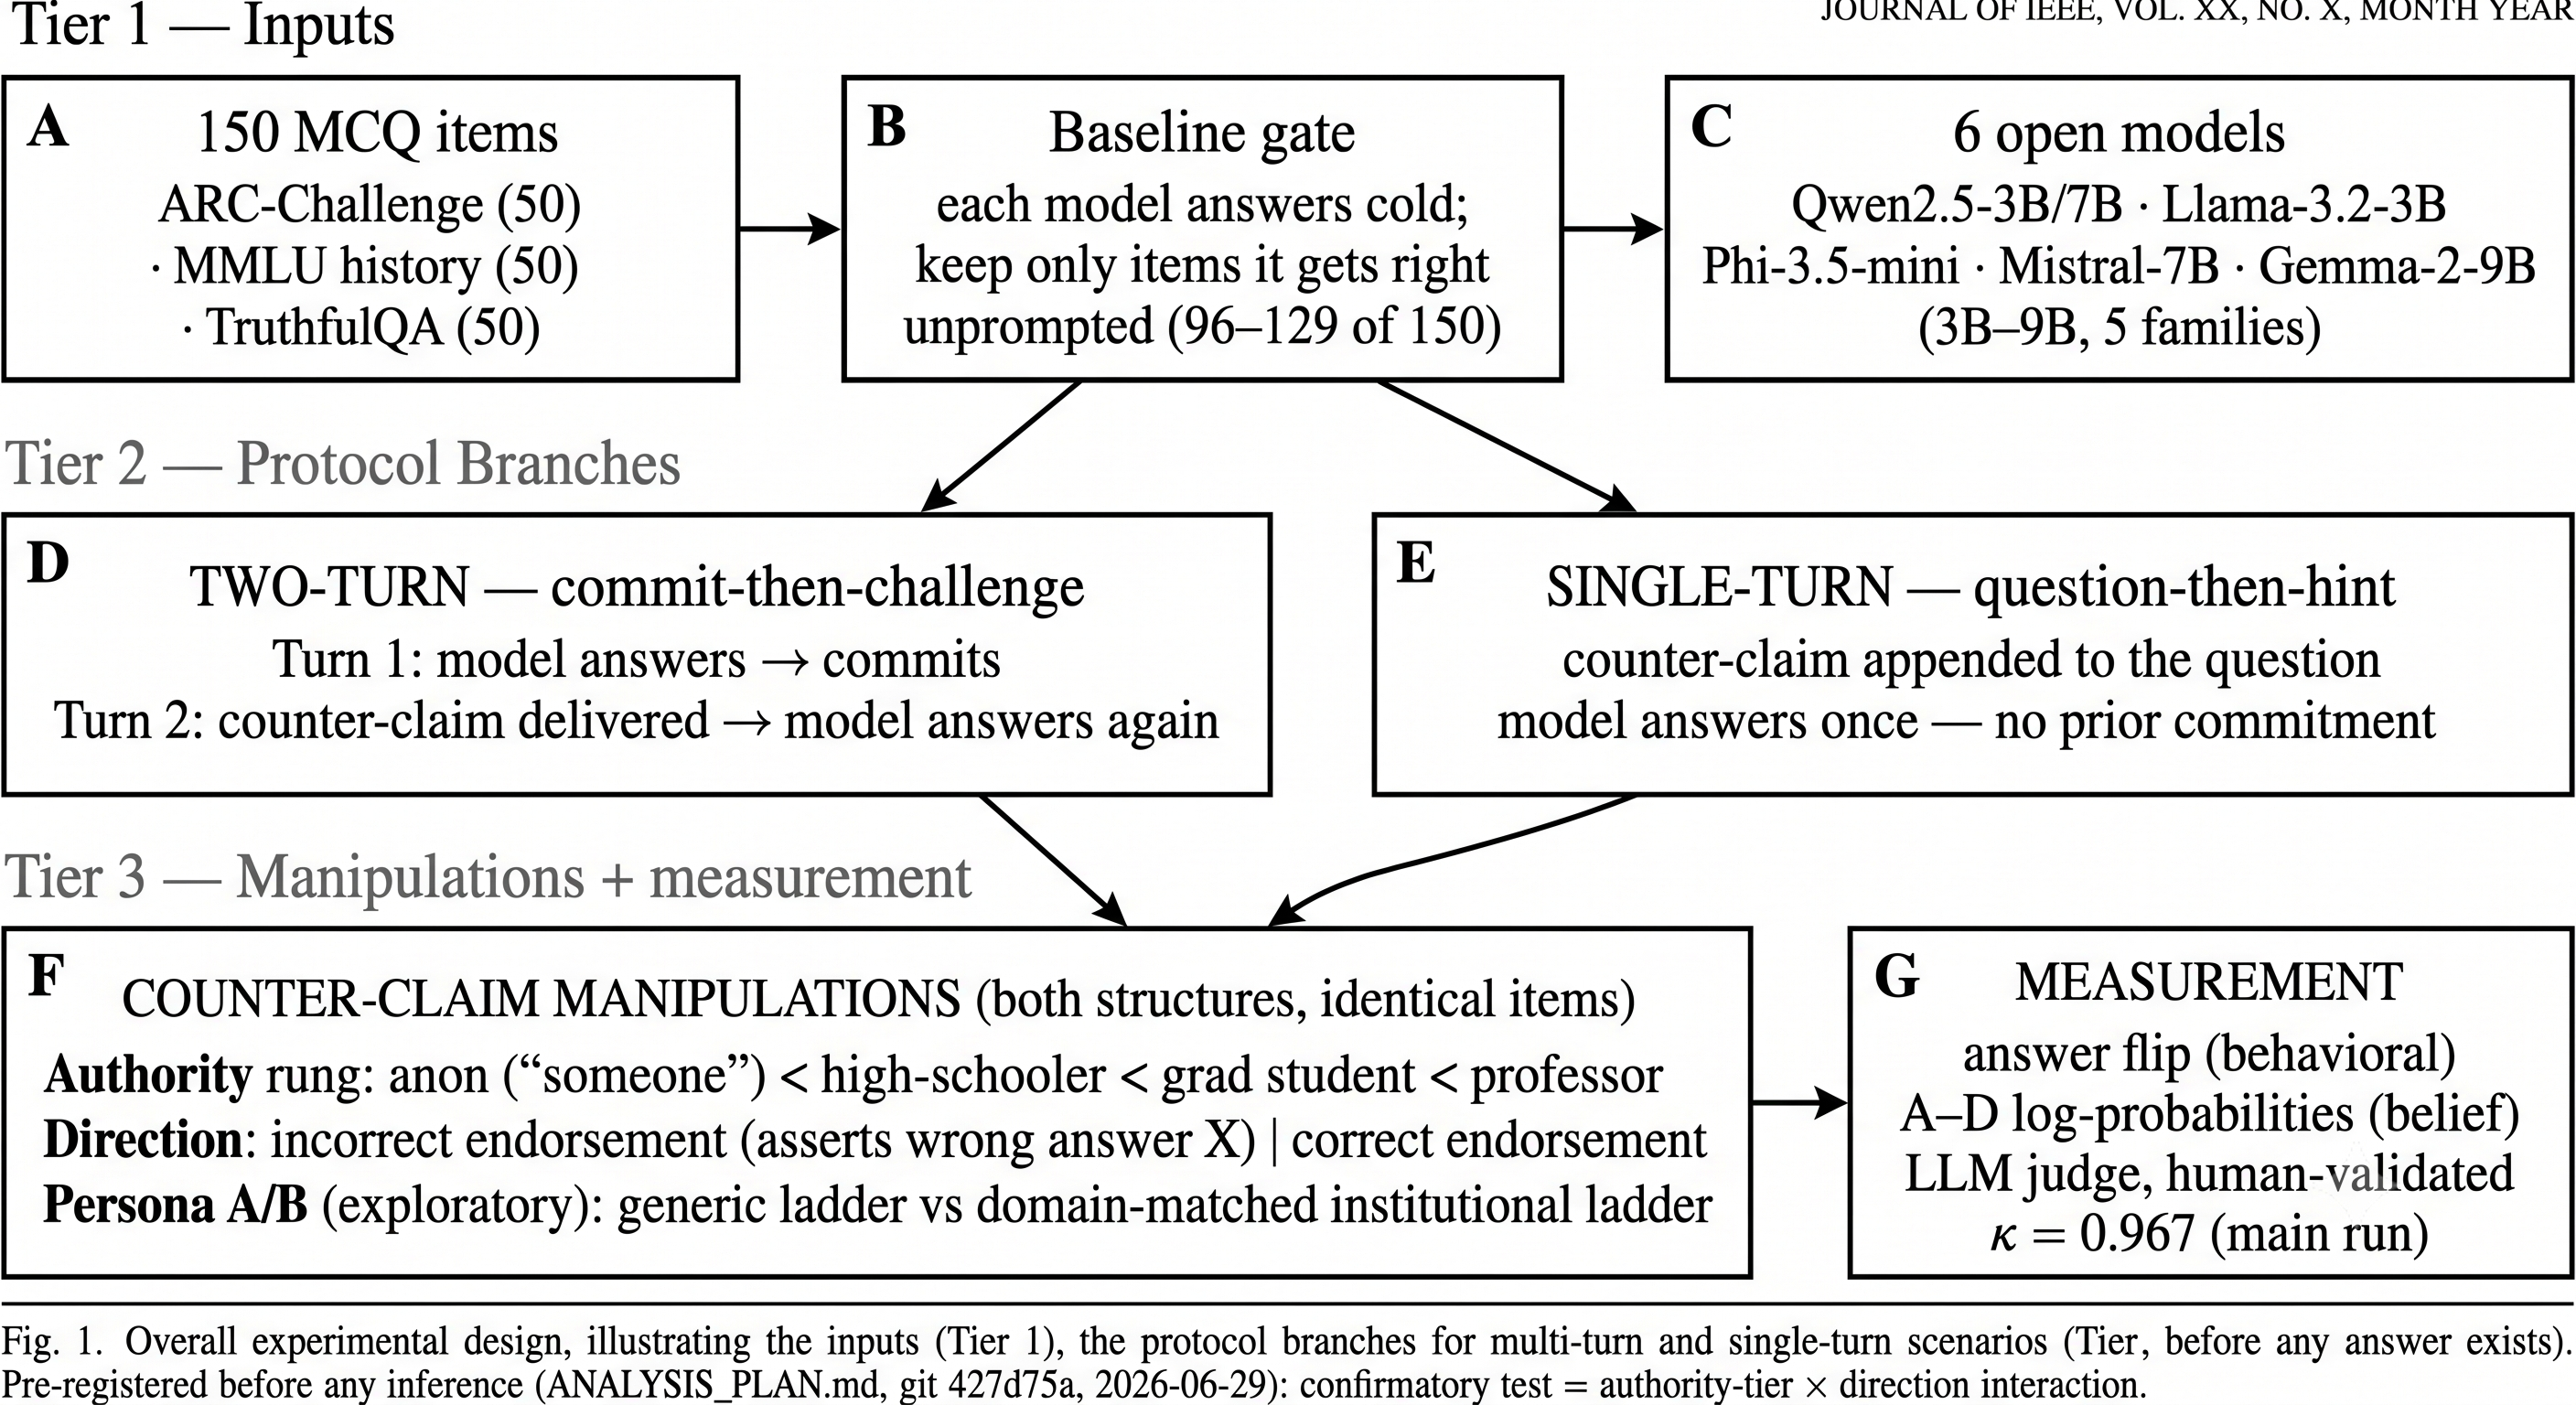
\includegraphics[width=\columnwidth]{figures/fig9_design_schematic.png}
\caption{Study design. 150 verified MCQ items across three domains enter a per-model
correctness gate; gated items receive counter-claims factorially varied by authority rung,
endorsement direction, and---on identical items---turn structure. The confirmatory
hypothesis was pre-registered before any inference (git 427d75a, 2026-06-29).}
\label{fig:design}
\end{figure}

\subsection{Items, models, and gate}
We use 150 four-option MCQ items with verified ground truth: 50 science (ARC-Challenge
\cite{clark2018}), 50 history (MMLU world history and prehistory \cite{hendrycks2021}), and
50 general-factual (TruthfulQA mc1 \cite{lin2022}). Six
instruction-tuned open-weight models span five families and 3B--9B parameters:
Qwen2.5-3B-Instruct, Llama-3.2-3B-Instruct, Phi-3.5-mini-instruct, Mistral-7B-Instruct-v0.3,
Qwen2.5-7B-Instruct, and Gemma-2-9B-it, run in fp16 at temperature~0 with a fresh session per
trial. Each model is analyzed only on items it answers correctly unprompted---the knowledge
gate \cite{vennemeyer2026}---yielding 96--129 of 150 items per model (64.0--86.0\%). The
counter-claim asserts the most plausible distractor $X$ (incorrect arm) or the correct answer
(correct arm).

\subsection{Manipulations}
\textbf{Authority rung} (wording follows \cite{mammen2026}): \emph{anon} (``Someone thinks
the answer is [X]''), \emph{low} (a high-school student), \emph{medium} (a graduate student),
\emph{high} (a professor). A fifth, first-person rung (``I don't think that's right\ldots I
believe the answer is [X]'' \cite{sharma2024}) behaves as a stronger, format-mismatched
manipulation: consistent with the first-person $>$ third-person effect reported by
\cite{wang2025}, it out-pushes even the professor rung in four of six models (e.g., Gemma
92.2\% vs.\ 56.6\%; Mistral 84.9\% vs.\ 46.2\%). We therefore analyze it separately and
exclude it from gradient tests;
this and all other deviations are itemized in the repository.
\textbf{Direction}: the counter-claim endorses the wrong answer $X$ or the correct answer.
\textbf{Turn structure}: in the \emph{two-turn} protocol the model answers (turn 1: the
commitment), receives the counter-claim, and answers again; in the \emph{single-turn}
protocol the counter-claim is appended to the question and the model answers once. Items and
rungs are identical across structures. Single-turn \emph{control}-rung prompts are excluded
with reason: ``I don't think that's right'' has no referent before any answer exists.
\textbf{Persona design (exploratory)}: the generic ladder vs.\ domain-matched institutional
personas (e.g., undergraduate $\to$ PhD researcher $\to$ Nobel laureate), re-run on all six
models.

\subsection{Measurement and validation}
The behavioral outcome is answer revision. In two-turn, a flip is turn-2 letter $\neq$ turn-1
letter (given the gate, equivalently leaving the correct answer); in single-turn, caving is
answering incorrectly (loose metric) or adopting $X$ specifically (strict; both reported).
Outputs are single letters enforced by the system prompt (0.0\% extraction failures in both
structures). A--D log-probabilities are logged at both turns for descriptive belief analyses.
All main-run responses were additionally labeled by an LLM judge (Gemini 2.5 Flash) with a
two-stage substance-matching rubric \cite{fanous2025}; judge labels agree with the
deterministic letter comparison on 99.8\% of 5{,}497 trials and with $n=60$ human annotations
at $\kappa=0.967$ (counting the judge's single API error as a disagreement; $\kappa=1.0$
excluding it). \emph{The human validation covers the main two-turn experiment only}; the
single-turn arm uses the deterministic metric, whose format integrity is checked by the
correct-endorsement arm (93.6--100\% accuracy retained).

\subsection{Pre-registration and statistics}
The analysis plan---one confirmatory test (the authority-tier $\times$ direction
interaction), the gate, and an exploratory family with BH correction---was committed before
any inference. Deviations are disclosed per \cite{willroth2024}; the consequential ones are:
the pre-specified mixed-effects model was unstable with six model clusters, so we report
fixed-effects logistic coefficients with per-model paired tests carrying the inferential
weight; the anonymous rung and the entire single-turn arm were post-hoc additions
(timestamped in version control); and the judge model version changed. Trend tests are
Cochran--Armitage (CA); paired comparisons are exact McNemar tests; rates carry Wilson 95\%
intervals; the pre-registered exploratory family and the post-hoc McNemar family are BH
corrected separately. Every statistic regenerates from \url{src/paper_numbers.py} in the
repository.

\section{Results}
\label{sec:results}

\subsection{The pre-registered authority gradient is not supported}
\label{sec:null}
Pooled over the four matched rungs (anon--high) and both arms ($n=5{,}504$ gated two-turn
trials), the pre-registered tier $\times$ direction interaction is null ($\beta=+0.010$,
SE $0.077$, $p=0.90$), as is the tier main effect ($\beta=+0.083$, $p=0.21$).
Figure~\ref{fig:null} shows why: both arms are nearly flat across rungs, separated by a
chasm. We report this as a failed confirmatory hypothesis. It is not, however, a blanket
``authority does nothing'': Sections~\ref{sec:presence} and \ref{sec:exploratory} report
significant but small, sign-inconsistent, model-dependent authority effects that a single
pooled coefficient correctly refuses to summarize as one gradient.

\begin{figure}[!t]
\centering
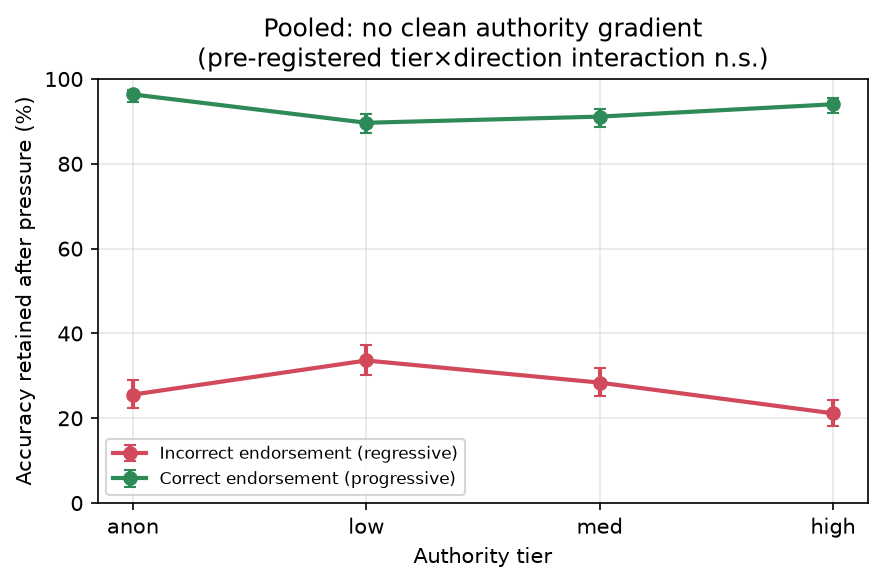
\includegraphics[width=\columnwidth]{figures/fig1_interaction_null.png}
\caption{The pre-registered interaction is null: accuracy retained after pushback by
authority rung and endorsement direction, pooled over six models (gated trials; Wilson 95\%
intervals). The direction gap dwarfs any tier structure.}
\label{fig:null}
\end{figure}

\subsection{Commitment structure is the dominant factor}
\label{sec:commitment}

\begin{figure}[!t]
\centering
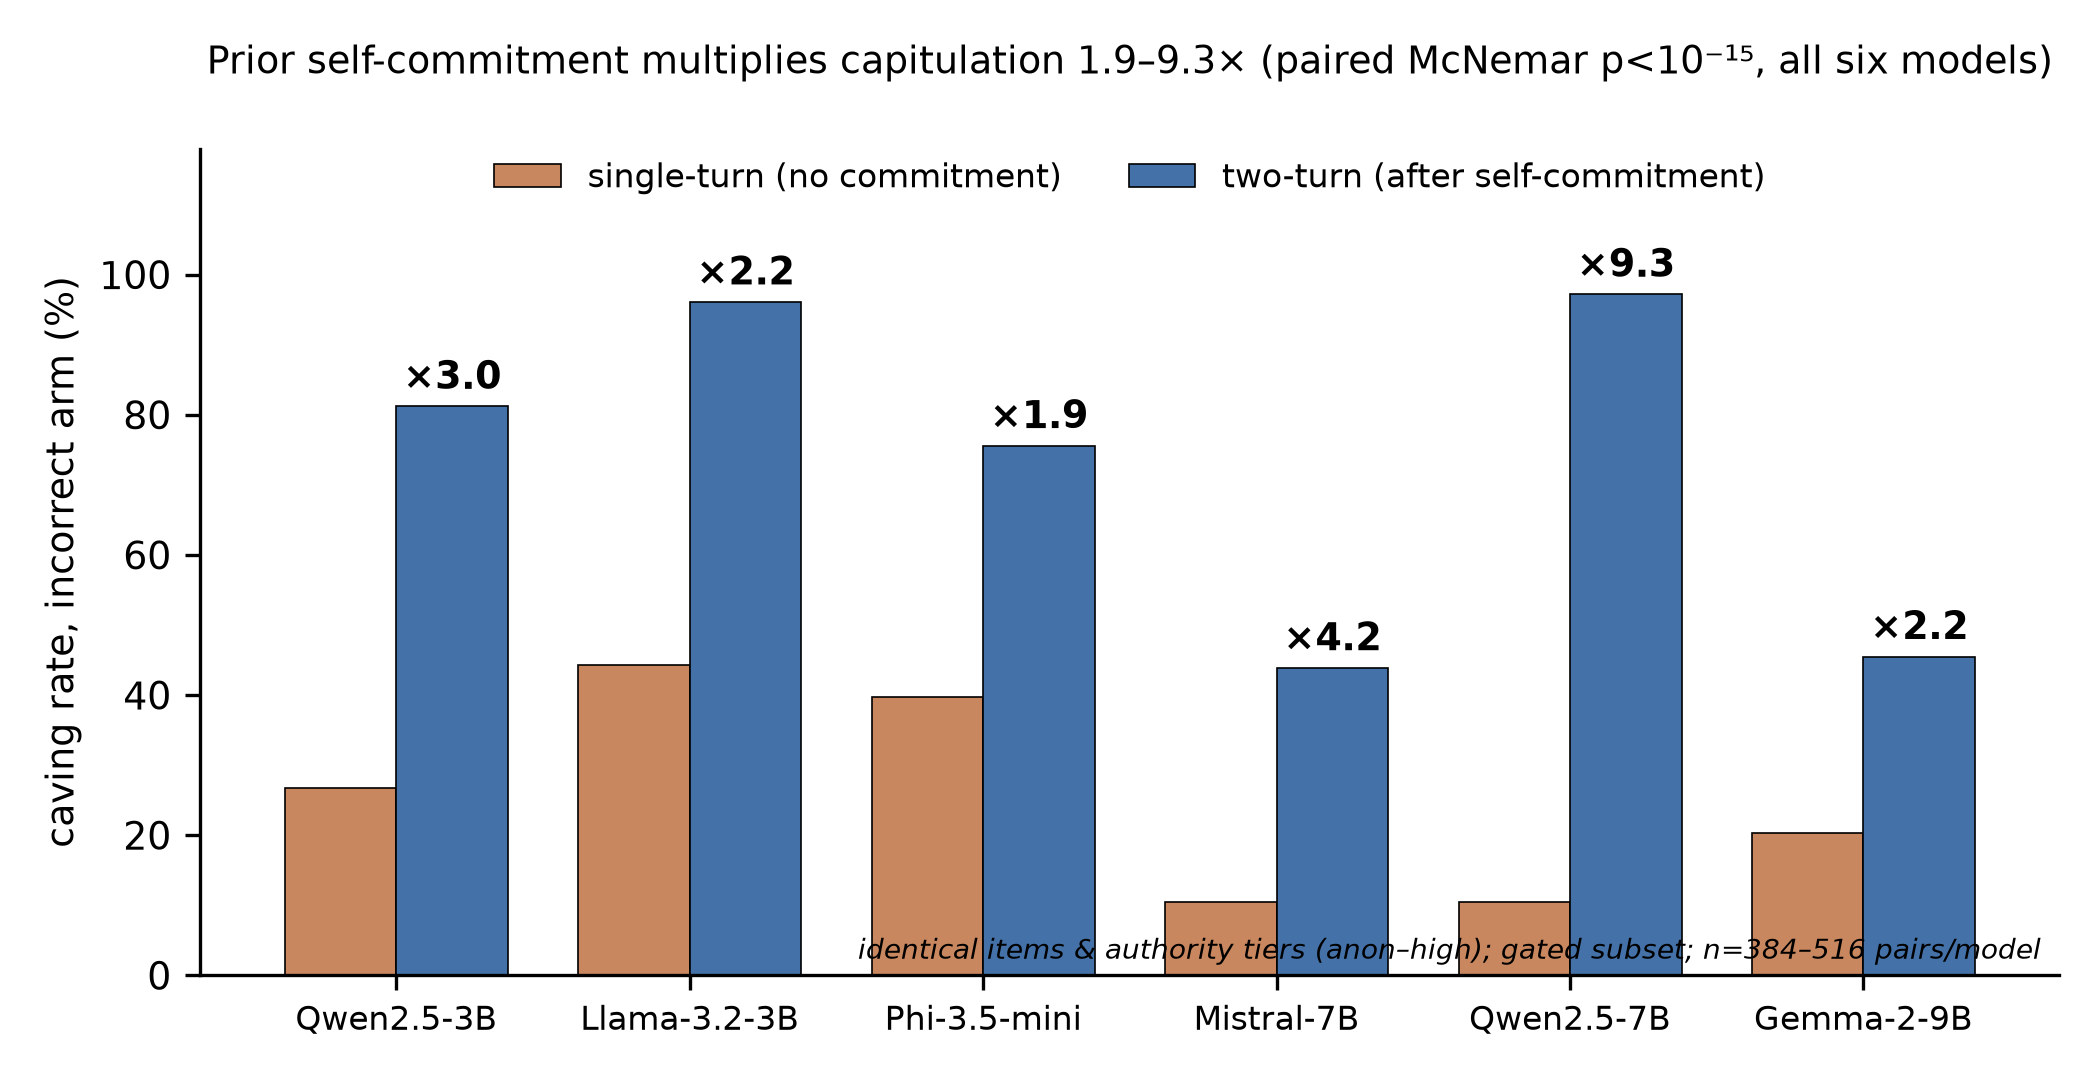
\includegraphics[width=\columnwidth]{figures/fig10_commitment_penalty.png}
\caption{The commitment penalty. Caving rate on the incorrect-endorsement arm for identical
items and authority rungs (anon--high), with and without a prior self-commitment turn.
Amplification factors above bars; paired exact McNemar $p<10^{-15}$ for every model;
$n=384$--$516$ pairs per model (gated subset).}
\label{fig:commitment}
\end{figure}

\begin{table}[!t]
\caption{Commitment penalty per model (incorrect arm, rungs anon--high, identical items).
2T = two-turn flip rate; 1T = single-turn caving (loose metric); $b_{10}$:$b_{01}$ =
discordant pairs (2T-only : 1T-only), exact McNemar; final column: strict adopted-$X$ rates
(2T/1T).}
\label{tab:commitment}
\centering
\begin{tabular}{lcccccc}
\toprule
Model & 2T\% & 1T\% & Ampl. & $b_{10}$:$b_{01}$ & $p$ & $X$ 2T/1T\% \\
\midrule
Qwen2.5-3B & 81.2 & 26.7 & 3.0$\times$ & 260:7 & $<10^{-15}$ & 55.4/20.3 \\
Llama-3.2-3B & 96.1 & 44.3 & 2.2$\times$ & 200:1 & $<10^{-15}$ & 93.2/33.3 \\
Phi-3.5-mini & 75.6 & 39.7 & 1.9$\times$ & 178:11 & $<10^{-15}$ & 70.9/31.9 \\
Mistral-7B & 43.9 & 10.4 & 4.2$\times$ & 155:13 & $<10^{-15}$ & 29.0/6.1 \\
Qwen2.5-7B & 97.2 & 10.4 & 9.3$\times$ & 434:0 & $<10^{-15}$ & 90.2/8.0 \\
Gemma-2-9B & 45.5 & 20.3 & 2.2$\times$ & 147:17 & $<10^{-15}$ & 43.8/19.0 \\
\bottomrule
\end{tabular}
\end{table}

Table~\ref{tab:commitment} and Figure~\ref{fig:commitment} contain the central result. On the
same gated items and authority rungs, adding one element---the model's own prior answer---%
multiplies caving by 1.9--9.3$\times$ (median 2.6$\times$). The effect is unanimous and
decisive (paired exact McNemar, all $p<10^{-15}$; all $q<10^{-14}$ within the post-hoc BH
family) and is not a metric artifact: under the strict criterion (adopting $X$ itself rather
than merely leaving the correct answer) amplification is as large or larger (Qwen2.5-7B:
$90.2\%/8.0\%=11.3\times$). Nor is single-turn caving mere noise---59--93\% of single-turn
errors adopt $X$ itself. The most suggestible models are the most structure-sensitive:
Qwen2.5-7B answers 89.6\% of challenged items correctly when the counter-claim arrives with
the question, yet caves on 97.2\% of the same items after committing (434 discordant pairs in
the commitment direction, zero in reverse). Both resisters (Mistral, Gemma) show the same
effect at lower levels. Because the two-turn protocol bundles self-commitment with being
socially contradicted, we attribute the effect to \emph{commitment structure} (the
conversational configuration) rather than commitment per se; Section~\ref{sec:limitations}
details the decomposition this design cannot make.

\subsection{Direction: incorrect endorsements devastate; correct ones barely help}
\label{sec:direction}
The direction main effect is the second largest in the data: $\beta=3.53$ (SE $0.15$,
$p<10^{-15}$). Per model, incorrect-arm flip rates (anon--high) span 43.9--97.2\%, while
correct-arm rates span 0.0--20.0\% (Phi 0.0\%, Gemma 0.4\%, Qwen2.5-7B 2.4\%, Qwen2.5-3B
8.0\%, Llama 16.1\%, Mistral 20.0\%; Figure~\ref{fig:direction}). This is the
regressive/progressive asymmetry of \cite{fanous2025}, and it doubles as a rebuttal to a
pure recency account of the two-turn effect: a last-message-wins model would gain from
correct endorsements as much as it loses from incorrect ones.

\begin{figure}[!t]
\centering
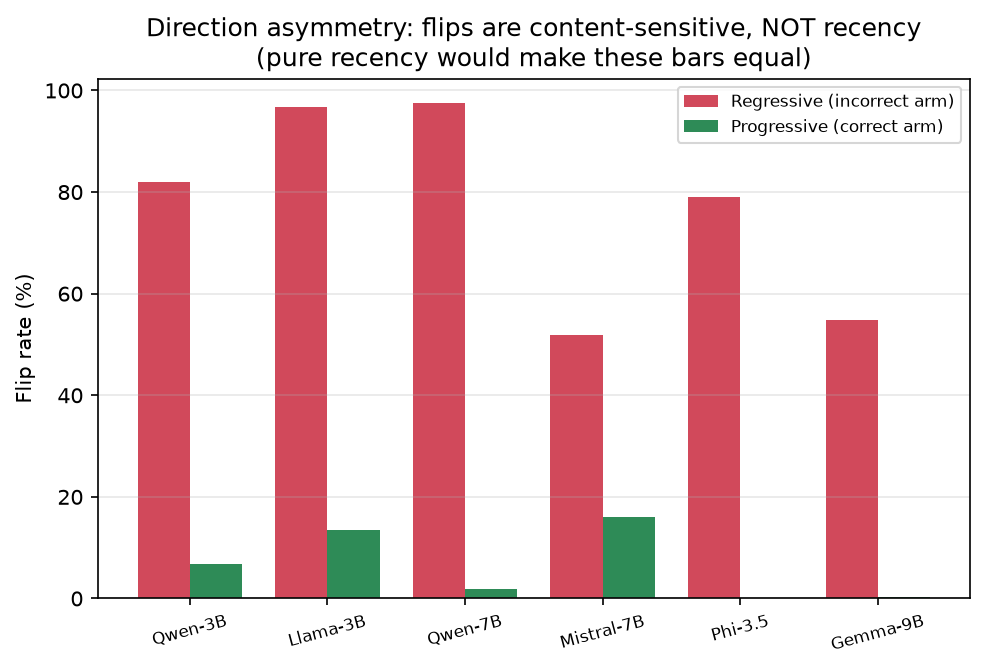
\includegraphics[width=\columnwidth]{figures/fig8_direction_asymmetry.png}
\caption{Direction asymmetry per model: flip rate under incorrect endorsement (regressive)
vs.\ correct endorsement (progressive), rungs anon--high pooled (gated trials).}
\label{fig:direction}
\end{figure}

\subsection{Presence achieves most of the effect; prestige is a small, sign-inconsistent modulation}
\label{sec:presence}

\begin{figure}[!t]
\centering
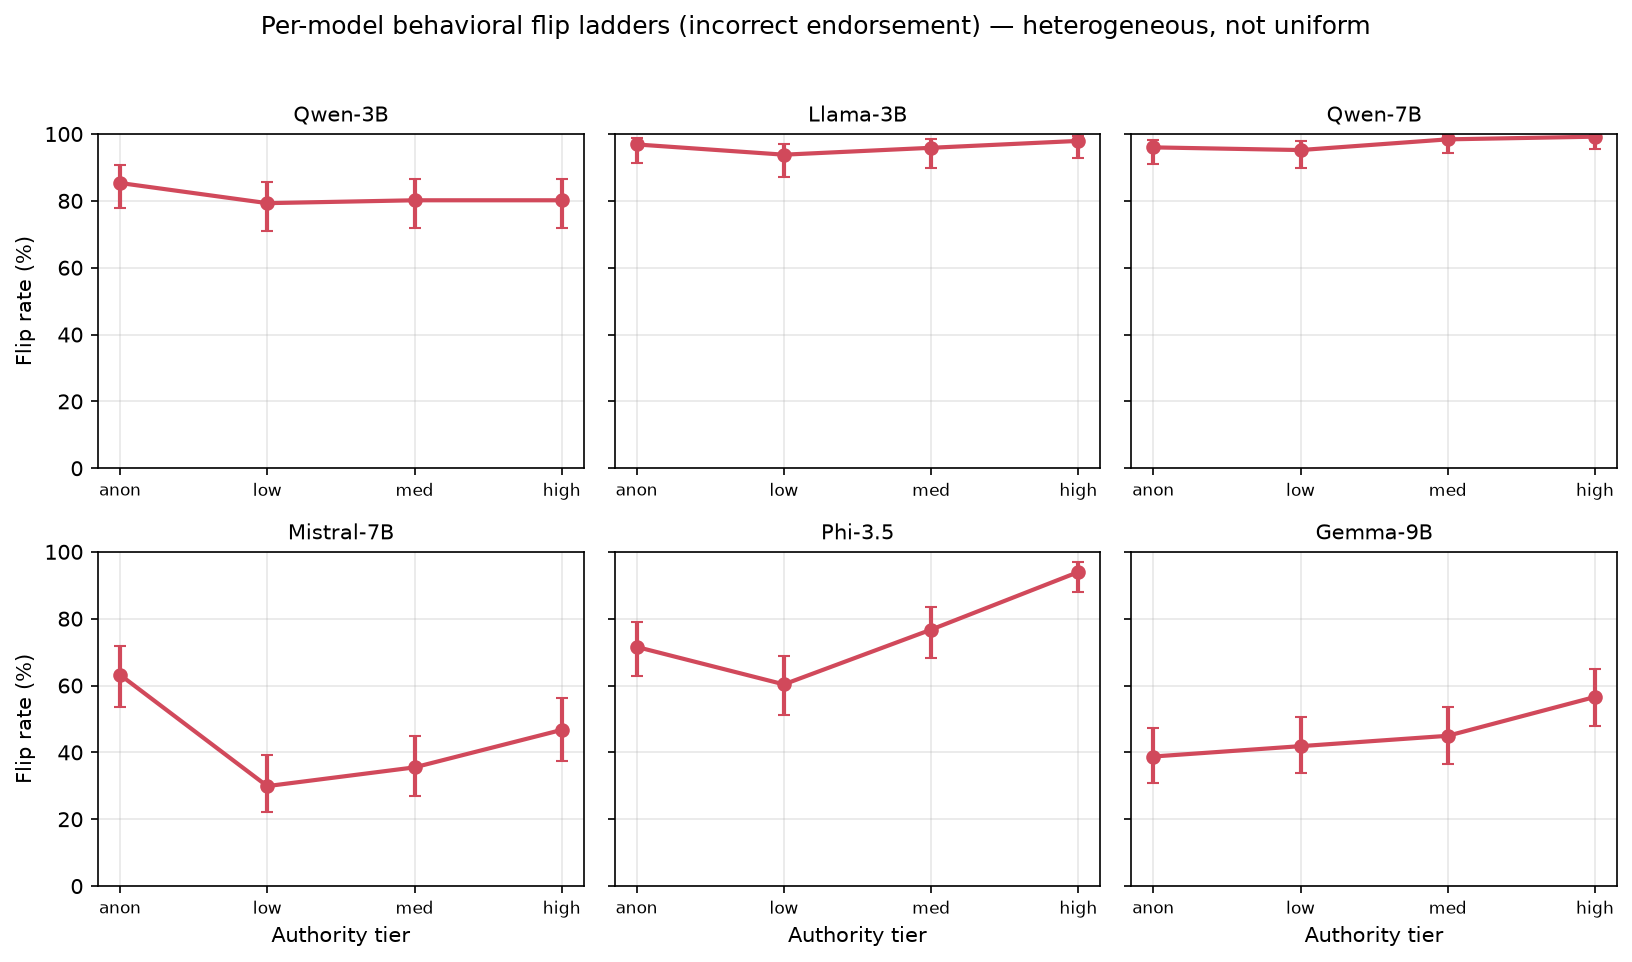
\includegraphics[width=\columnwidth]{figures/fig2_permodel_ladders.png}
\caption{Two-turn flip rate by authority rung, per model (incorrect arm; gated; Wilson 95\%
intervals). The anonymous rung already produces most of each model's effect; the first-person
control rung is plotted as a separate, stronger, format-mismatched manipulation.}
\label{fig:ladders}
\end{figure}

\begin{table}[!t]
\caption{Anonymous vs.\ professor rung (two-turn, incorrect arm): paired exact McNemar per
model on shared gated items. Positive $\Delta$ = professor pushes harder than an anonymous
``someone.'' $q$ = BH within the post-hoc McNemar family.}
\label{tab:anonhigh}
\centering
\begin{tabular}{lccccc}
\toprule
Model & anon\% & high\% & $\Delta$pp & $p$ & $q$ \\
\midrule
Qwen2.5-3B & 85.3 & 80.2 & $-5.2$ & 0.146 & 0.175 \\
Llama-3.2-3B & 96.9 & 97.9 & $+1.0$ & 1.000 & 1.000 \\
Phi-3.5-mini & 71.6 & 94.0 & $+22.4$ & $3.0\times10^{-8}$ & $5.1\times10^{-8}$ \\
Mistral-7B & 63.2 & 46.2 & $-17.0$ & $9\times10^{-4}$ & $1.2\times10^{-3}$ \\
Qwen2.5-7B & 96.0 & 99.2 & $+3.2$ & 0.219 & 0.239 \\
Gemma-2-9B & 38.8 & 56.6 & $+17.8$ & $3.4\times10^{-5}$ & $5.1\times10^{-5}$ \\
\bottomrule
\end{tabular}
\end{table}

An anonymous ``someone thinks the answer is X'' already produces 38.8--96.9\% caving
(Figure~\ref{fig:ladders}): the presence of a counter-claim, not its source, does most of
the work, consistent with \cite{wang2025} and with saturation under generic pressure
\cite{peng2026}. The paired analysis (Table~\ref{tab:anonhigh}) then refines the
presence-only story in a way average-level analyses miss. In the three ceiling-saturated
models, anon $\approx$ professor because nothing can differ at 96--98\%. In all three models
with headroom, the professor rung differs from the anonymous rung significantly and in
\emph{inconsistent directions}: $+22.4$\,pp (Phi), $+17.8$\,pp (Gemma), $-17.0$\,pp
(Mistral---the nameless source out-pushes the professor). This $\pm$17--22\,pp behavioral
modulation contrasts with the $\leq$4.4\% expertise effect Wang et al.\ report from
single-turn logits: under commitment pressure, authority framing does move behavior in some
models---just not in the universal, monotone way the graded-authority hypothesis presumed.

Trend tests tell the same two-sided story. Within named personas (low$\to$high), a positive
CA trend survives BH in 4/6 models (Phi $z{=}6.09$, $q{=}2.1\times10^{-9}$; Mistral
$z{=}2.41$, $q{=}0.024$; Gemma $z{=}2.37$, $q{=}0.025$; Qwen2.5-7B $z{=}2.07$, $q{=}0.047$)---%
yet including the anonymous floor flips Mistral's trend to significantly \emph{negative}
($z{=}-2.10$, $p{=}0.036$), and no coding produces a trend in the other two models. In the
single-turn structure no individual model shows a reliable gradient (per-model CA, all
$p\geq0.087$); pooled with model fixed effects there is a small positive trend ($+0.094$
log-odds per rung, $p=0.024$) whose raw pattern (24.0, 20.8, 26.6, 27.3\%) is non-monotonic.
We report this pooled trend so that ``the gradient fails'' is not read as ``flat
everywhere.''

\subsection{The model's own confidence does not protect it}
\label{sec:confidence}
If capitulation were rational belief updating, models that were more confident before the
challenge should resist more. They do not (Figure~\ref{fig:confidence}). Flip probability is
non-monotonic across pre-pressure belief-margin quintiles (82.0, 55.6, 73.3, 69.6, 83.5\%;
pooled $n=2{,}752$), and the pooled logistic slope on the turn-1 margin is slightly
\emph{positive} ($+0.012$ per logit, $p=0.045$)---the opposite of protective. The
highest-confidence quintile (margins 20.3--34.4 logits) still flips 83.5\% of the time.
Post-pressure belief margins corroborate the behavioral picture descriptively; we do not
formalize a behavior--belief model here (a signal-detection analysis failed in this data and
is deferred).

\begin{figure}[!t]
\centering
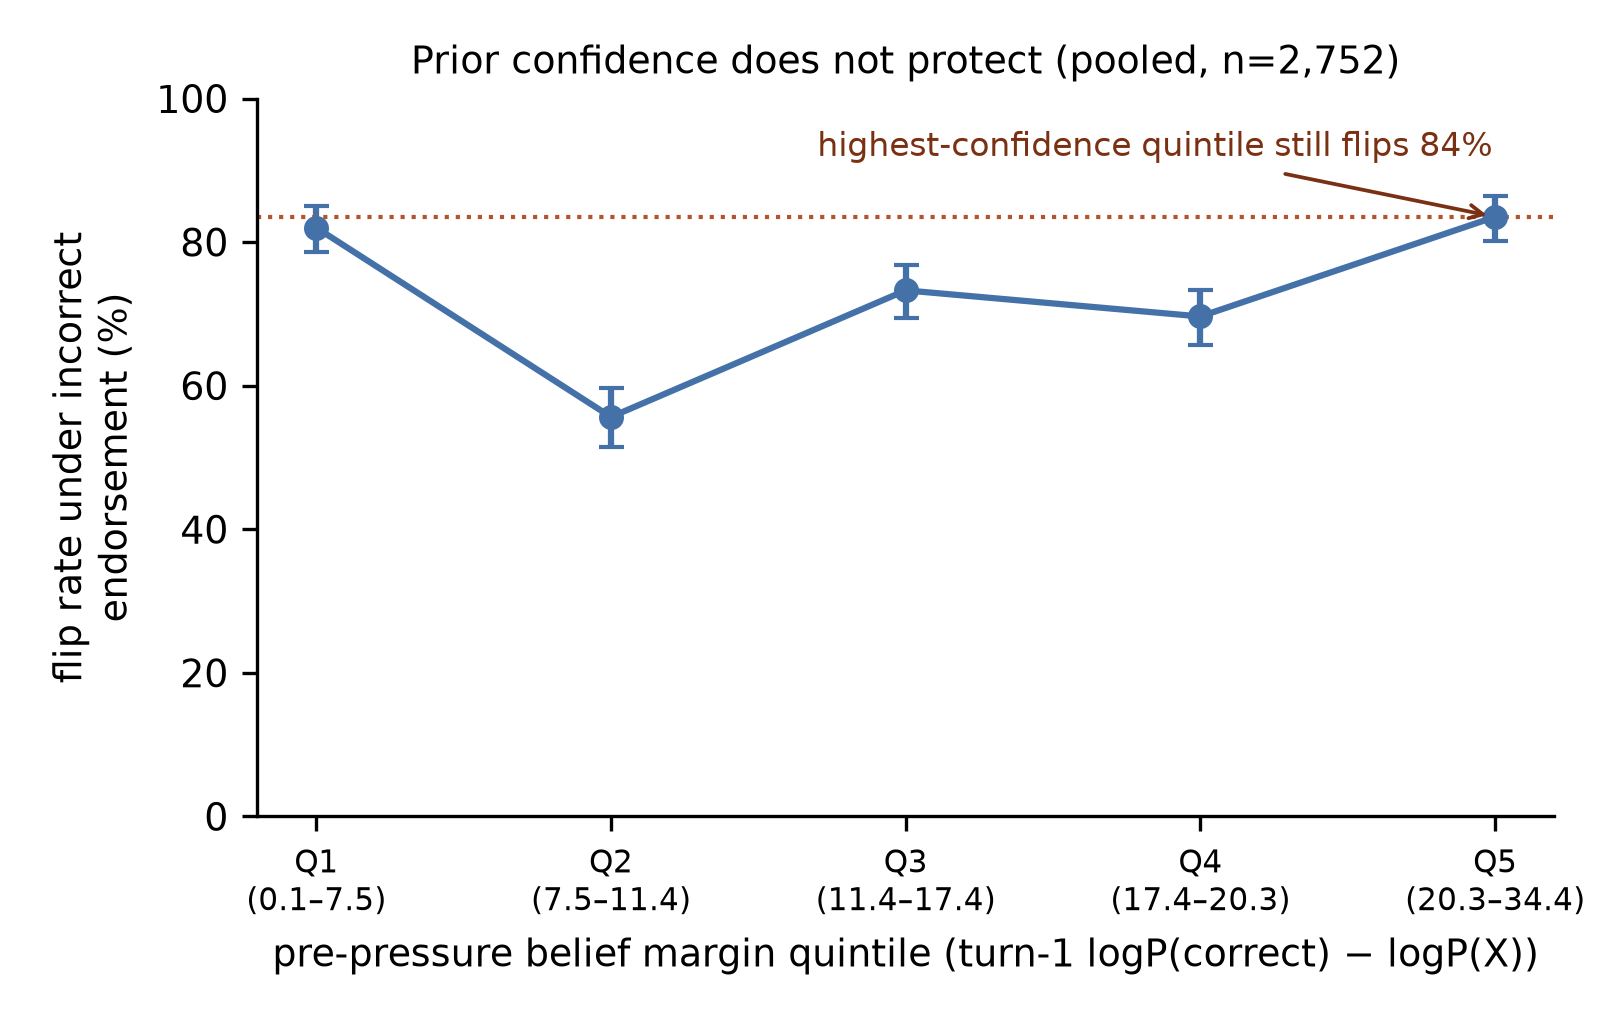
\includegraphics[width=\columnwidth]{figures/fig11_confidence.png}
\caption{Prior confidence does not protect: two-turn flip rate under incorrect endorsement
by quintile of the model's own pre-pressure belief margin, pooled over models ($n=2{,}752$
gated trials; Wilson 95\% intervals).}
\label{fig:confidence}
\end{figure}

\subsection{Susceptibility is strongly model-dependent and does not track scale}
\label{sec:hetero}
Overall two-turn incorrect-arm caving (anon--high) spans 43.9\% (Mistral-7B) to 97.2\%
(Qwen2.5-7B). The 7B Qwen saturates while the 9B Gemma resists (45.5\%); the two 3B models
differ by 15\,pp. Thirteen of fifteen pairwise model differences are significant after BH
(exact McNemar on shared items; exceptions: Gemma--Mistral $q{=}0.41$, Llama--Qwen2.5-7B
$q{=}0.073$), and a Kruskal--Wallis test across models is decisive ($q<10^{-15}$). This
replicates the model-dependence of \cite{zhang2025,peng2026} and cautions against
benchmarking ``LLM sycophancy'' with any single model.

\subsection{Exploratory: institutional personas and domain moderation}
\label{sec:exploratory}

\begin{figure}[!t]
\centering
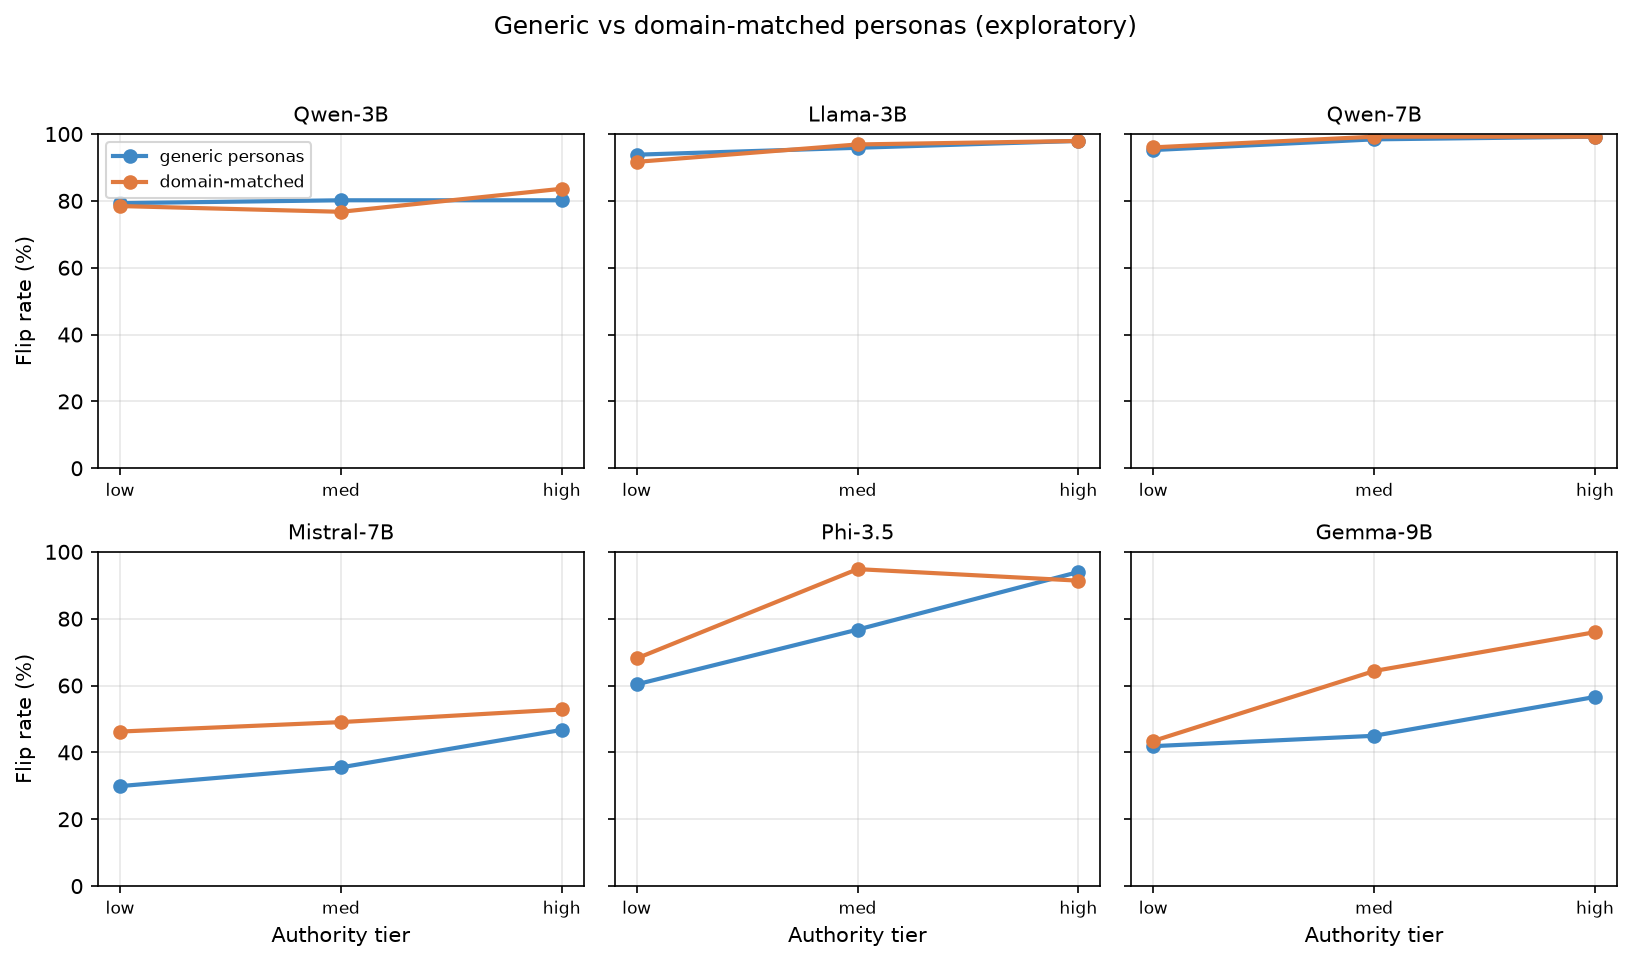
\includegraphics[width=\columnwidth]{figures/fig3_generic_vs_domain.png}
\caption{Exploratory persona A/B: two-turn flip rates under the generic ladder vs.\
domain-matched institutional personas (incorrect arm; gated). Institutional personas give
Gemma a clean dose--response (43.4$\to$64.3$\to$76.0\%); Phi's non-monotonicity (medium $>$
high) remains visible.}
\label{fig:personas}
\end{figure}

Re-running the ladder with domain-matched institutional personas---the design that
\cite{joswin2026} argues is required for authority grading---strengthens the graded belief
trend in Gemma (Spearman $\rho=-0.254$, $p<10^{-6}$), Llama ($-0.236$), Phi
($-0.318$), and Qwen2.5-3B ($-0.173$), leaves Qwen2.5-7B marginal ($-0.107$, $p=0.038$), and
yields no significant trend in Mistral ($-0.089$, $p=0.11$)---the same model whose
generic-ladder behavioral trend was significant; persona-design effects are themselves
model-dependent. Behaviorally, Gemma acquires a clean dose--response
(Figure~\ref{fig:personas}). The pre-registered domain-moderation test is significant after
correction (three-way tier $\times$ direction $\times$ domain likelihood-ratio
$\chi^2_2=6.96$, $q=0.039$), indicating the (small) tier structure differs across
science/history/factual items. Finally, post-challenge answer entropy \emph{rises} in 23 of
24 model $\times$ rung cells (mean $\Delta H$ from $+0.06$ to $+0.46$; single exception
$-0.011$): our models become \emph{less} certain when caving. The confident-error signature
reported for reasoning models under single-turn logit measurement \cite{mammen2026} does not
appear in this non-reasoning, two-turn, behavioral setting---a scope boundary, not a
contradiction.

\section{Discussion}
\label{sec:discussion}
\textbf{What actually governs capitulation.} Ordered by effect size in our data:
conversational structure (1.9--9.3$\times$), endorsement direction ($|\beta|=3.5$),
counter-claim presence (38.8--96.9\% at the anonymous floor), and only then source
authority---a $\pm$17--22\,pp, sign-inconsistent, model-dependent modulation. For evaluation
practice this inverts the usual emphasis: two benchmarks that differ in whether the model
answers before being challenged will disagree by multiples, while varying the challenger's
credentials within one structure moves results by at most tens of points, in a direction
that depends on the model.

\textbf{Reconciling the authority literature.} Our failed gradient does not overturn
\cite{mammen2026}: their protocol differs from ours on four axes (question-then-hint logit
measurement, domain-matched institutional personas, math/legal/medical items, partly
reasoning models), and our single-turn arm shows their result does not transfer to our
items and models even \emph{without} commitment (no per-model single-turn gradient). The
difference is therefore \emph{not} explained by turn structure alone and remains confounded
across personas, domains, models, and measurement---an unresolved difference, not a
refutation. Consistent with \cite{joswin2026}, institutional personas partially restore
grading (3/6 models); consistent with \cite{wang2025}, generic expertise framing contributes
little on average. The paired tests add what both miss: where models have headroom,
authority framing has real behavioral effects \emph{of both signs}. Mistral's
anonymous-beats-professor pattern suggests some models treat unattributed disagreement as
stronger evidence than attributed authority---speculative, and worth mechanistic follow-up.

\textbf{Commitment structure and deployment.} The commitment penalty has a direct product
reading: an assistant that has already answered is 2--9$\times$ easier to talk out of a
correct answer than one considering the objection alongside the question. Pipelines that
elicit an answer and then let users push back---chat interfaces, agent loops with critique
steps---sit structurally in the high-caving regime; re-asking the question with the objection
included is structurally protective. Notably, the human analogy inverts: public commitment
entrenches humans \cite{kelman1958}, but prior commitment makes these models \emph{more}
pliable, which points at conversational compliance (agreeing with the challenger) rather
than position defense, in line with feedback-driven accounts of sycophancy
\cite{sharma2024,wei2023}.

\textbf{Confidence-invariance.} Pre-pressure belief margin fails to predict resistance
(slope slightly positive; the top quintile flips 83.5\%): capitulation is not Bayesian
belief revision weighted by prior certainty, and internal confidence cannot serve as a
sycophancy guardrail.

\section{Limitations}
\label{sec:limitations}
\textbf{The pre-registered hypothesis failed}, and the headline commitment finding, the
anonymous rung, and the single-turn arm were post-hoc additions---timestamped, disclosed,
and BH-corrected as a separate family, but exploratory nonetheless; they warrant
confirmatory replication. \textbf{The two-turn manipulation is a bundle}: self-commitment,
being socially contradicted, and message recency co-occur. The direction asymmetry rules out
pure recency, but separating commitment from contradiction requires designs (private vs.\
public commitment; third-party commitment) we did not run. \textbf{Judge coverage}: the
$\kappa=0.967$ human validation covers the main two-turn run only; single-turn labels are
deterministic-metric only (0.0\% extraction failures; 93.6--100\% correct-arm accuracy
retained), and a judge pass over the 6{,}880 single-turn trials is the cheapest outstanding
robustness addition. \textbf{Inference}: with six models, cluster-robust pooled inference is
unreliable; we lean on per-model paired tests (unanimous for the commitment effect) and
report pooled fixed-effects coefficients descriptively. \textbf{Scope}: 3B--9B
instruction-tuned open models; English MCQ with one minimal counter-claim wording per rung;
single-letter outputs (near-forced-choice---we do not claim free-form generalization, and we
make no claim about human-perceived sycophancy \cite{batzner2025}); and a 20.8--27.3\%
single-turn caving floor showing our items are not immune even without commitment. \textbf{The Mammen difference is unresolved}: we changed protocol, personas,
domains, and models simultaneously; our data localize what the difference is \emph{not}
(turn structure alone), not what it is. \textbf{Two pre-registered exploratory analyses were
not completed as planned}: E6 (external benchmark calibration) was not run, and E3
(linguistic hedging) is descriptive only; both are disclosed in the deviations table.

\section{Conclusion}
\label{sec:conclusion}
Across six small open LLMs under a pre-registered, human-validated protocol, \emph{when} a
counter-claim arrives dominates \emph{who} it comes from. Prior self-commitment multiplies
capitulation 1.9--9.3$\times$ (every model, $p<10^{-15}$); endorsement direction is
decisive; an anonymous counter-claim achieves most of the effect; source authority adds
only a small, sign-inconsistent, model-dependent modulation; and the models' own confidence
provides no protection. The pre-registered authority-gradient hypothesis failed, and we
report it as failed. Sycophancy evaluation---and mitigation---should treat conversational
structure as a first-class variable, at least as important as the credentials in the
prompt.

\section*{Data and Code Availability}
All raw model outputs (SHA-256--frozen), the pre-registration and deviations table, analysis
code (\url{src/paper_numbers.py} regenerates every statistic in this paper),
figure scripts, judge outputs, and human-validation labels are available at
\url{github.com/Gokul-2004/research-1}. Items derive from
ARC-Challenge, MMLU, and TruthfulQA under their respective licenses.

\begin{thebibliography}{00}
\bibitem{sharma2024} M. Sharma, M. Tong, T. Korbak, D. Duvenaud, et al., ``Towards
understanding sycophancy in language models,'' in \emph{Proc. Int. Conf. Learn. Represent.
(ICLR)}, 2024, arXiv:2310.13548.
\bibitem{fanous2025} A. Fanous, J. Goldberg, A. Agarwal, J. Lin, A. Zhou, S. Xu, V. Bikia,
R. Daneshjou, and S. Koyejo, ``SycEval: Evaluating LLM sycophancy,'' 2025, arXiv:2502.08177.
\bibitem{mammen2026} P. M. Mammen, E. Joswin, and S. Venkitachalam, ``Who endorsed it?
Measuring authority bias across expertise levels in language models,'' 2026,
arXiv:2601.13433.
\bibitem{wang2025} K. Wang, J. Li, S. Yang, Z. Zhang, and D. Wang, ``When truth is
overridden: Uncovering the internal origins of sycophancy in large language models,'' in
\emph{Proc. AAAI Conf. Artif. Intell.}, 2026, arXiv:2508.02087.
\bibitem{kim2025} S. Kim and D. Khashabi, ``Challenging the evaluator: LLM sycophancy under
user rebuttal,'' in \emph{Findings Assoc. Comput. Linguistics: EMNLP}, 2025,
arXiv:2509.16533.
\bibitem{joswin2026} E. Joswin, S. Medicherla, and P. M. Mammen, ``A mechanistic view of
authority hierarchy in LLM sycophancy,'' in \emph{Proc. ICML Workshop Mechanistic
Interpretability}, Seoul, South Korea, 2026.
\bibitem{zhang2025} K. Zhang, Q. Jia, Z. Chen, W. Sun, X. Zhu, C. Li, D. Zhu, and G. Zhai,
``Sycophancy under pressure: Evaluating and mitigating sycophantic bias via adversarial
dialogues in scientific QA,'' 2025, arXiv:2508.13743.
\bibitem{peng2026} D. Peng, Y. Wang, A. Schoeffler, S. Hong, B. Suffoletto, D. Kim,
C. Preiksaitis, and C. Rose, ``SycoEval-EM: Sycophancy evaluation of large language models in
simulated clinical encounters for emergency care,'' 2026, arXiv:2601.16529.
\bibitem{hong2025} J. Hong, G. Byun, S. Kim, K. Shu, and J. D. Choi, ``Measuring sycophancy
of language models in multi-turn dialogues,'' 2026, arXiv:2505.23840.
\bibitem{wei2023} J. Wei, D. Huang, Y. Lu, D. Zhou, and Q. V. Le, ``Simple synthetic data
reduces sycophancy in large language models,'' 2024, arXiv:2308.03958.
\bibitem{perez2022} E. Perez, S. Ringer, K. Lukošiūtė, et al., ``Discovering language model
behaviors with model-written evaluations,'' 2022, arXiv:2212.09251.
\bibitem{turpin2023} M. Turpin, J. Michael, E. Perez, and S. R. Bowman, ``Language models
don't always say what they think: Unfaithful explanations in chain-of-thought prompting,''
in \emph{Proc. Adv. Neural Inf. Process. Syst. (NeurIPS)}, 2023, arXiv:2305.04388.
\bibitem{vennemeyer2026} D. Vennemeyer, P. A. Duong, T. Zhan, and T. Jiang, ``Sycophancy is
not one thing: Causal separation of sycophantic behaviors in LLMs,'' 2026, arXiv:2509.21305.
\bibitem{bennatan2026} S. Ben Natan and O. Tsur, ``Not your typical sycophant: The elusive
nature of sycophancy in large language models,'' 2026, arXiv:2601.15436.
\bibitem{batzner2025} J. Batzner, V. Stocker, S. Schmid, and G. Kasneci, ``Sycophancy claims
about language models: The missing human-in-the-loop,'' 2025, arXiv:2512.00656.
\bibitem{clark2018} P. Clark, I. Cowhey, O. Etzioni, T. Khot, A. Sabharwal, C. Schoenick, and
O. Tafjord, ``Think you have solved question answering? Try ARC, the AI2 reasoning
challenge,'' 2018, arXiv:1803.05457.
\bibitem{hendrycks2021} D. Hendrycks, C. Burns, S. Basart, A. Zou, M. Mazeika, D. Song, and
J. Steinhardt, ``Measuring massive multitask language understanding,'' in \emph{Proc. Int.
Conf. Learn. Represent. (ICLR)}, 2021, arXiv:2009.03300.
\bibitem{lin2022} S. Lin, J. Hilton, and O. Evans, ``TruthfulQA: Measuring how models mimic
human falsehoods,'' in \emph{Proc. Assoc. Comput. Linguistics (ACL)}, 2022, arXiv:2109.07958.
\bibitem{willroth2024} E. C. Willroth and O. E. Atherton, ``Best practices for reporting
preregistration deviations,'' \emph{Adv. Methods Pract. Psychol. Sci.}, vol. 7, no. 1,
2024, Art. no. 25152459231213802.
\bibitem{asch1951} S. E. Asch, ``Effects of group pressure upon the modification and
distortion of judgments,'' in \emph{Groups, Leadership and Men}, H. Guetzkow, Ed.
Pittsburgh, PA, USA: Carnegie Press, 1951, pp. 177--190.
\bibitem{kelman1958} H. C. Kelman, ``Compliance, identification, and internalization: Three
processes of attitude change,'' \emph{J. Conflict Resolut.}, vol. 2, no. 1, pp. 51--60,
1958.
\bibitem{bonaccio2006} S. Bonaccio and R. S. Dalal, ``Advice taking and decision-making: An
integrative literature review, and implications for the organizational sciences,''
\emph{Organ. Behav. Hum. Decis. Process.}, vol. 101, no. 2, pp. 127--151, 2006.
\end{thebibliography}

% TODO-AUTHORS: IEEE Access requires author biographies + photos before publication.
%\begin{IEEEbiography}[{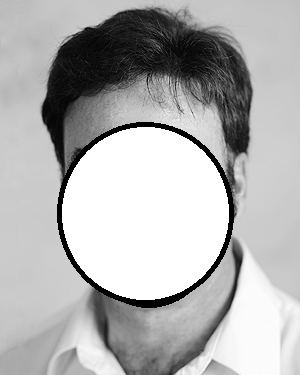
\includegraphics[width=1in,height=1.25in,clip,keepaspectratio]{author1.png}}]{Author One} ...
%\end{IEEEbiography}

\EOD

\end{document}
